\documentclass[letterpaper, 11 pt]{article}

\usepackage{fullpage}

\usepackage{graphics}
\usepackage{epsfig}
\usepackage{subfigure}
\usepackage{stfloats}
\usepackage{wrapfig}
%\title{\bf Proposal: Waypoint a Room with Simple Diff-Drive Robots}

\author{Kevin Kemper}

\begin{document}

\begin{flushright}
Kevin Kemper
\end{flushright}

\vspace{-2cm}
\begin{center}
\textbf{\huge ME537: Homework 1}
\end{center}


\thispagestyle{empty}
\pagestyle{empty}


%a. How does the number of hidden units impact the results?
%b. How does the training time impact the results?
%c. How does the learning rate impact the results?
%d. What other critical parameters impacted the results?

\begin{wrapfigure}{r}{0.5\textwidth}
	\centering
	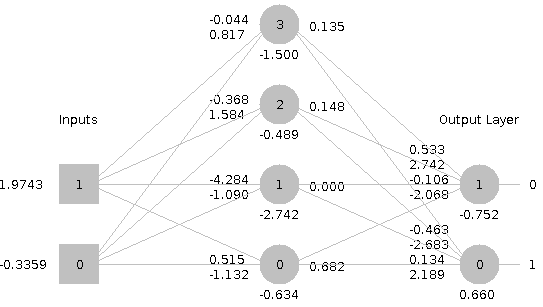
\includegraphics[scale=1.8]{../figures/Screenshot.png}
	\caption{\small	An example of the neural-network configuration showing inputs with
				resulting classification.
			}
	\label{fig:NNex}
\end{wrapfigure}

\vspace{0.5cm}
An example of the neural-network configuration is shown in figure \ref{fig:NNex}.
Values next to the squares indicate the input to the network.  Circles represent
"neurons" or nodes with values to the left indicating the weights associated
with attached inputs and values below indicating the constant weight.  Values to
the right of nodes indicate their output.  All nodes use sigmoid activation functions.
The outputs of the output nodes are thresholded to show final classification.

All results presented are averaged using 100 independent trials with error bars
indicating the standard deviation between trials. For every trial, the neural
network (NN) is trained over 500 epochs.  Each epoch consists of training the NN
over a random ordering of the training data followed by an evaluation using each
test case.  After the NN is evaluated with an input from the training data, the
weights are adjusting using gradient descent.

For all tests, there seems to be a point where the NN begins to over fit the training
data.  At that point the performance over the training data slowly reduces.  With
the data taken it cannot be determined if the classification error is monotonically
decreasing or converging to some equilibrium.  I would guess that it converges
to an equilibrium because the test data is at least related to the training data
so over-fitting should still capture most of the test data.

\section{Different amounts of hidden units}

The four graphs in figures \ref{fig:hTr}, \ref{fig:hT1}, \ref{fig:hT2} and \ref{fig:hT3}
demonstrate how the neural network evolves with various amounts of hidden units.
For each of the graphs, $\eta=0.01$.  From the results it seems that the minimum
number of hidden units necessary for the NN to converge within a reasonable number
of epochs is 3.  With 2 hidden units, the time for convergence is considerably longer
and has much larger variance in performance between trials.  Squinting carefully
at the graphs in figures \ref{fig:hTr}, \ref{fig:hT1}, \ref{fig:hT2} and \ref{fig:hT3},
we can see that over a sufficient number of epochs, 4 hidden units actually had
slightly less variance between trials than 5 hidden units when evaluated with the
test data.

\section{Different learning rates}

The second set of graphs in figures \ref{fig:eTr}, \ref{fig:eT1}, \ref{fig:eT2} and \ref{fig:eT3}
show the learning progression of a NN using 4 hidden units with 5 different learning rates.
The learning rates ($\eta$) used are equally spaced values between $0.001$ and $0.100$.
From the results there seems to be a threshold for choosing the best learning rate
located somewhere between $0.001$ and $0.026$.  For values close but slightly larger
than the threshold, the learning rate is acceptably fast and shows the least variance
between trials.  Figures \ref{fig:eTrex2} and \ref{fig:eT3ex2} are closeups of the
end of figures \ref{fig:eTr} and \ref{fig:eT3} respectively and serve to illustrate
how for both the training data and test data with $\eta=0.026$ the average correct
classification error percentage (CCP) was slightly less but produced less variance
between trials.



% eta=0.026 converged slightly slower but ended with much tighter variance between trials.

%perhaps over more epochs eta of 0.001 could have converged to a better set of weights.

\begin{figure}[bt]
	\centering
	\subfigure[Correct classification percentage over the training data.]{\label{fig:hTr}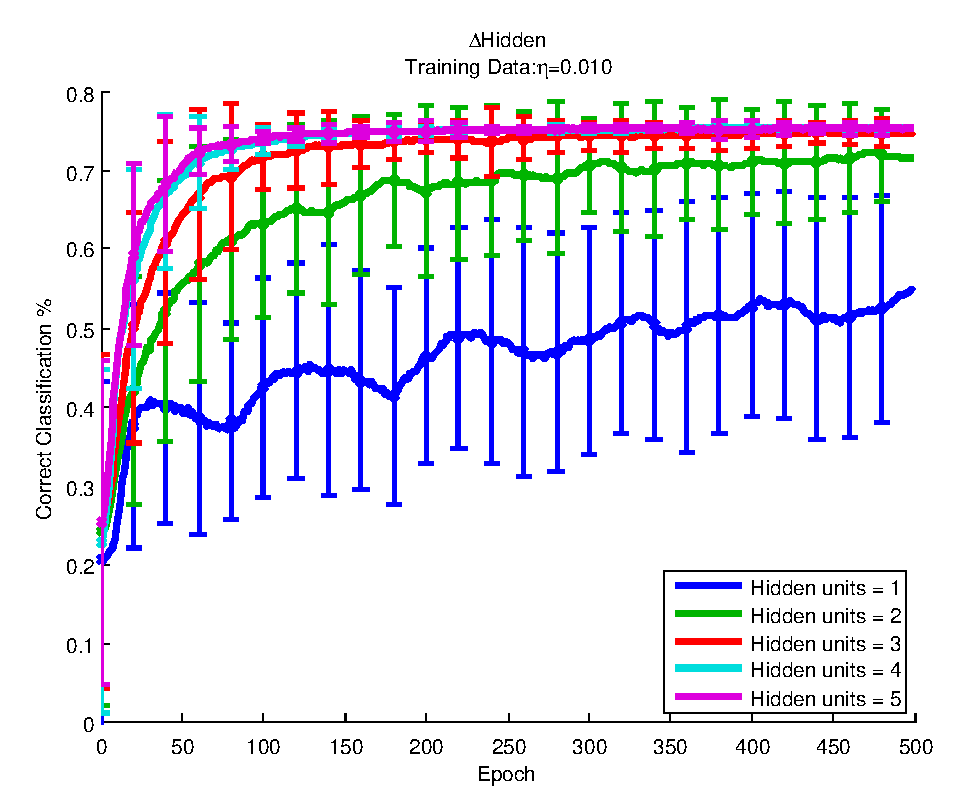
\includegraphics[scale=0.8]{../figures/hidden_train.pdf}}
	\subfigure[Correct classification percentage over test 1.]{\label{fig:hT1}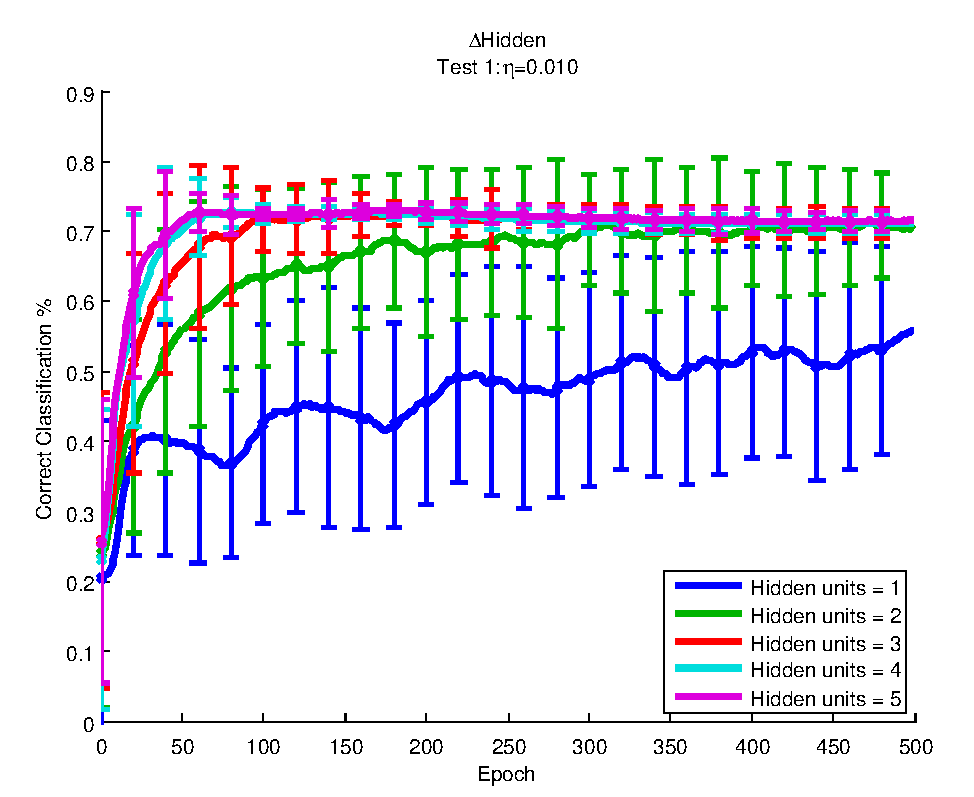
\includegraphics[scale=0.8]{../figures/hidden_test1.pdf}}
	\caption{	Performance of 5 neural-networks with the learning rate $\eta=0.01$.}
	\label{fig:h1}
\end{figure}

\begin{figure}[bt]
	\centering
	\subfigure[Correct classification percentage over test 2.]{\label{fig:hT2}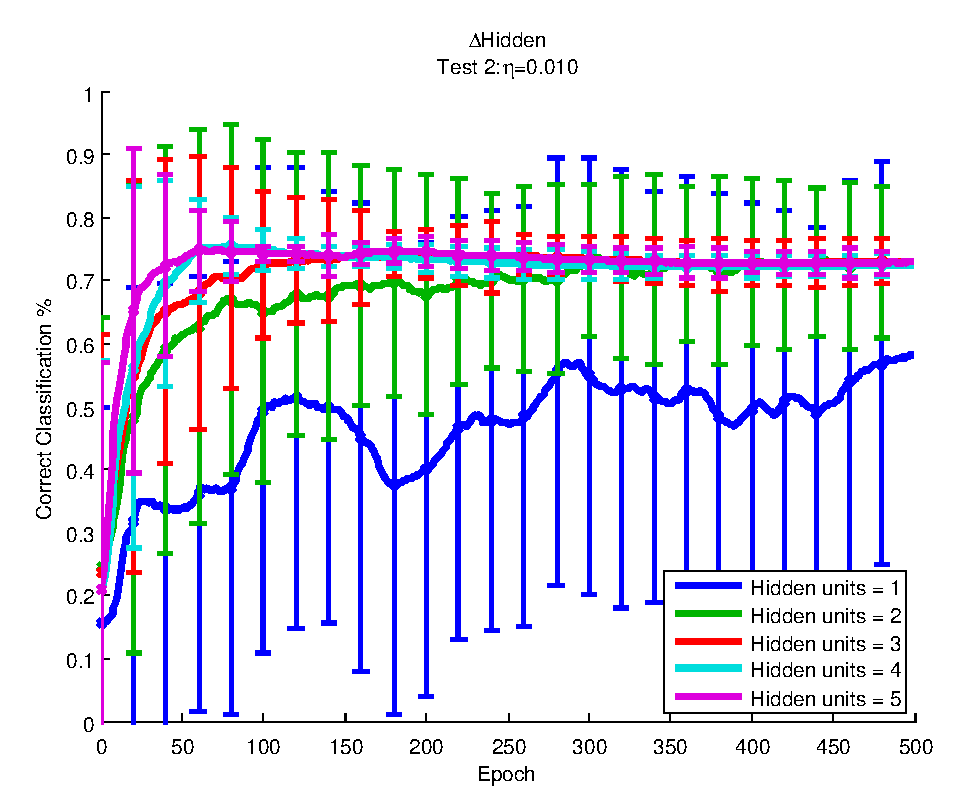
\includegraphics[scale=0.8]{../figures/hidden_test2.pdf}}
	\subfigure[Correct classification percentage over test 3]{\label{fig:hT3}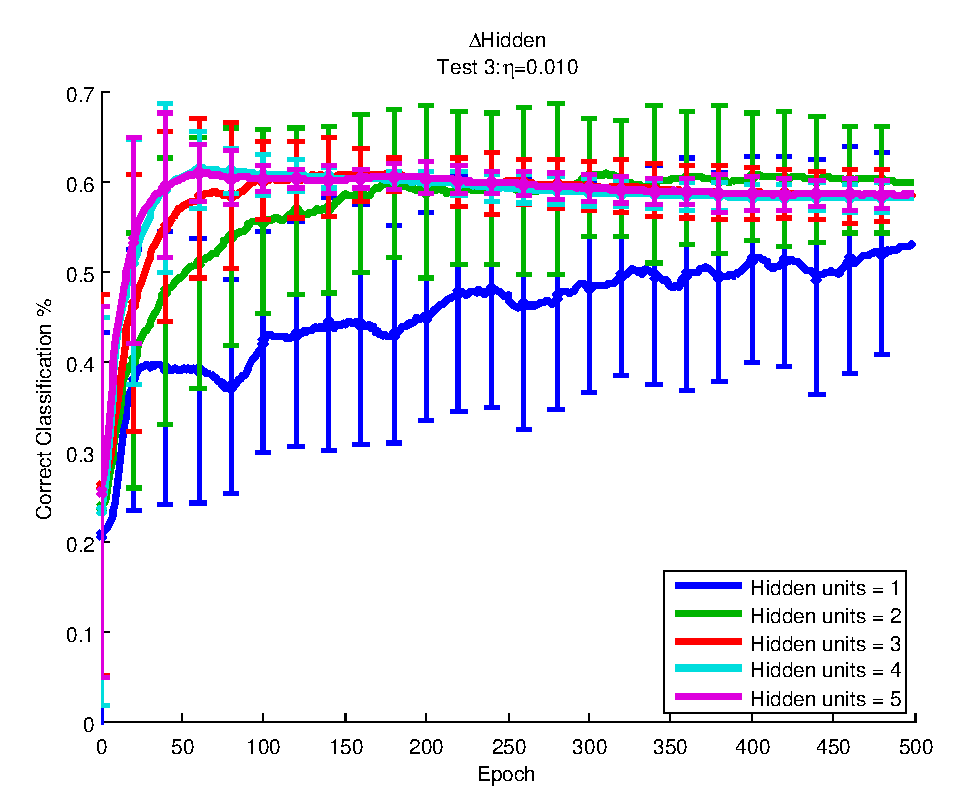
\includegraphics[scale=0.8]{../figures/hidden_test3.pdf}}
	\caption{	Performance of 5 neural-networks with the learning rate $\eta=0.01$.}
	\label{fig:h2}
\end{figure}



\begin{figure}[bt]
	\centering
	\subfigure[Correct classification percentage over the training data.]{\label{fig:eTr}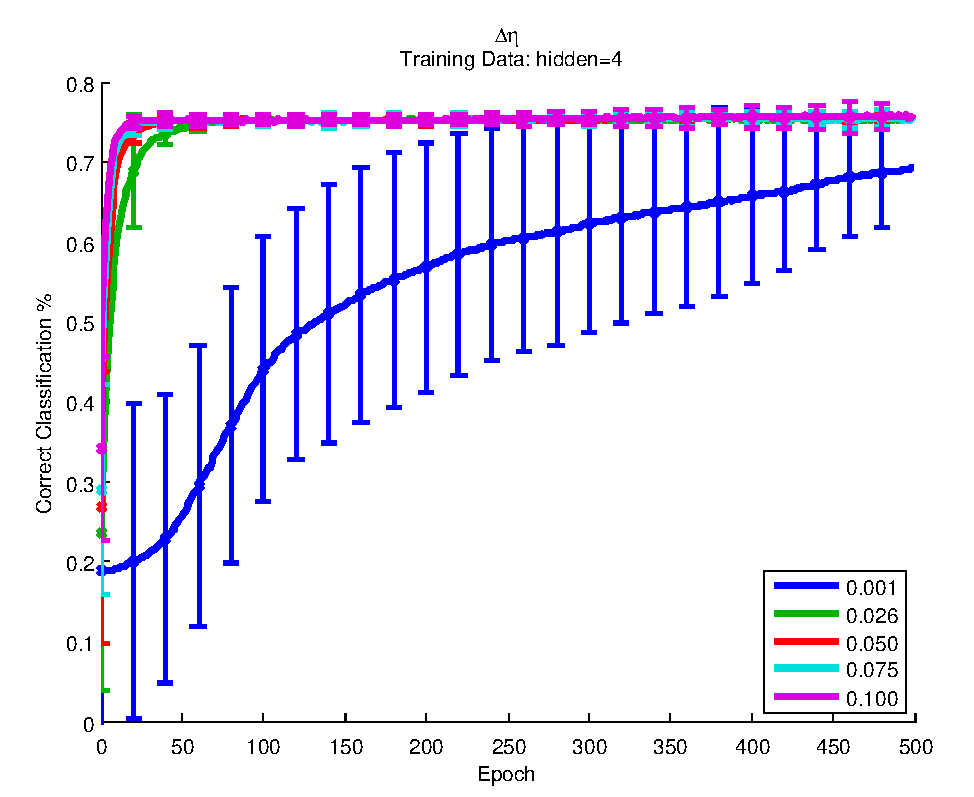
\includegraphics[scale=0.8]{../figures/eta_train.pdf}}
	\subfigure[Correct classification percentage over the test 1.]{\label{fig:eT1}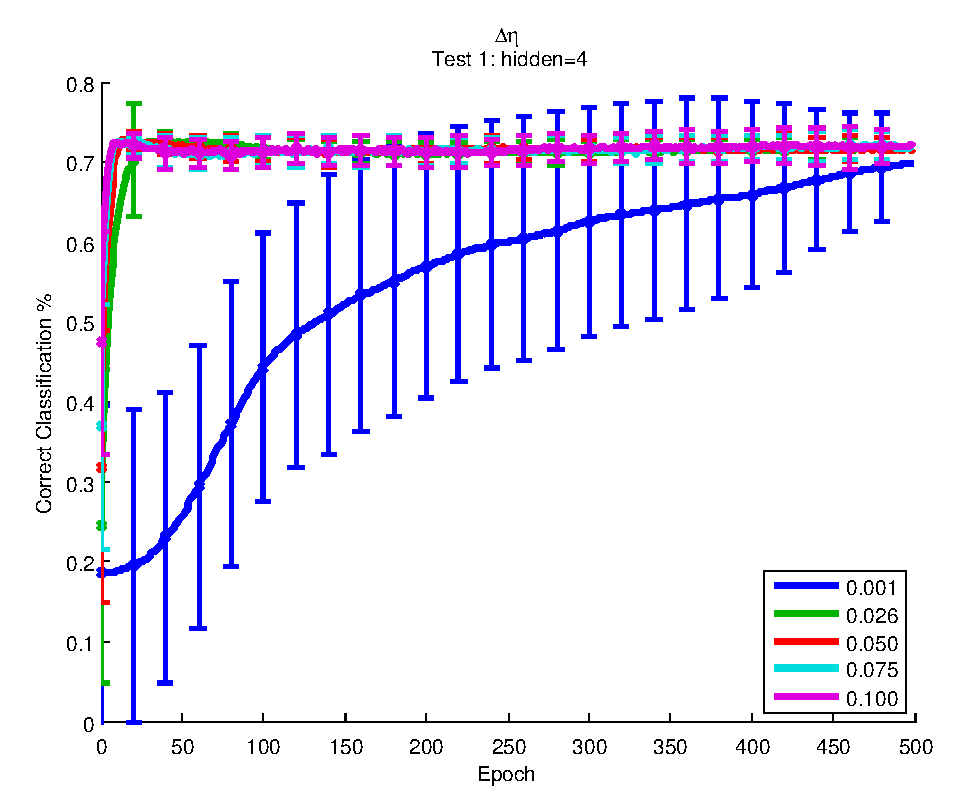
\includegraphics[scale=0.8]{../figures/eta_test1.pdf}}
	\caption{	Performance of a neural-network with 4 hidden units trained using different $\eta$ values.}
	\label{fig:e1}
\end{figure}

\begin{figure}[bt]
	\centering
	\subfigure[Correct classification percentage over the test 2.]{\label{fig:eT2}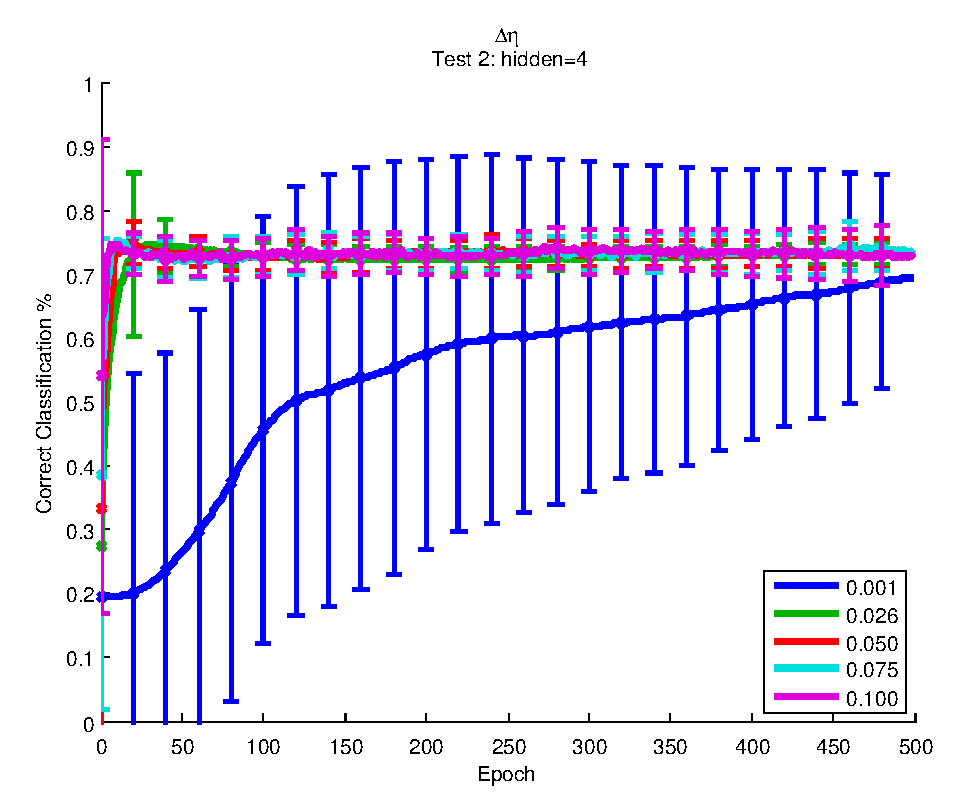
\includegraphics[scale=0.8]{../figures/eta_test2.pdf}}
	\subfigure[Correct classification percentage over the test 3.]{\label{fig:eT3}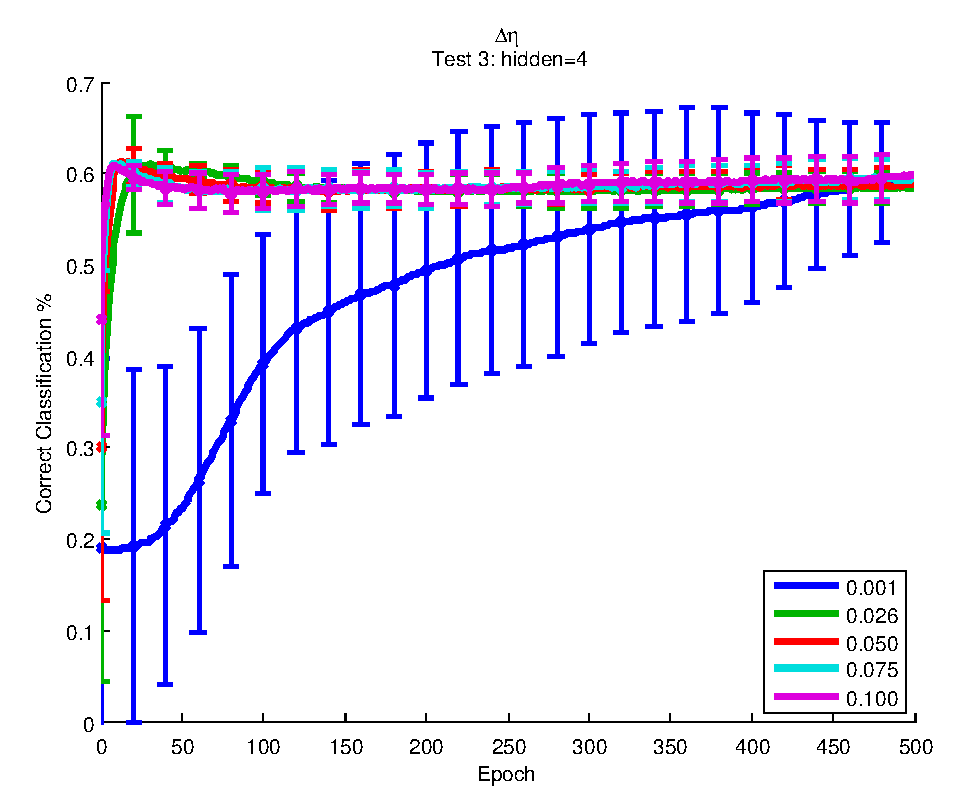
\includegraphics[scale=0.8]{../figures/eta_test3.pdf}}
	\caption{	Performance of a neural-network with 4 hidden units trained using different $\eta$ values.}
	\label{fig:e2}
\end{figure}


\begin{figure}[bt]
	\vspace{-2 cm}
	\centering
	\subfigure[Detail of the beginning of figure \ref{fig:eTr}.]{\label{fig:eTrex}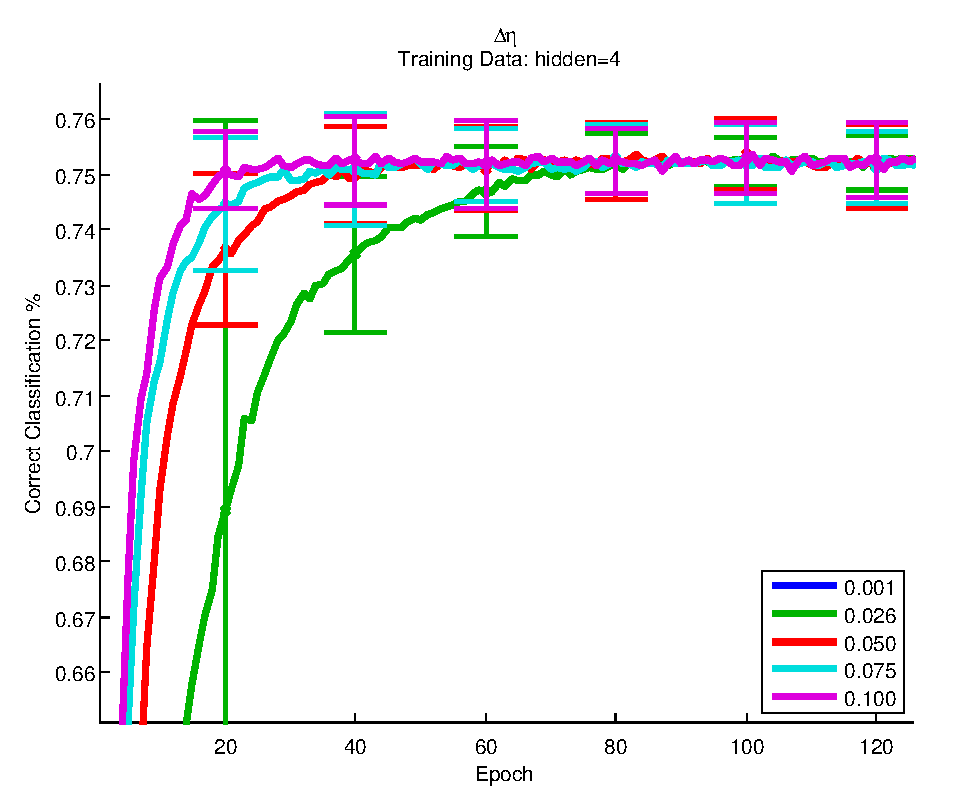
\includegraphics[scale=0.8]{../figures/eta_train_ex.pdf}}
	\subfigure[Detail of the end of figure \ref{fig:eTr}.]{\label{fig:eTrex2}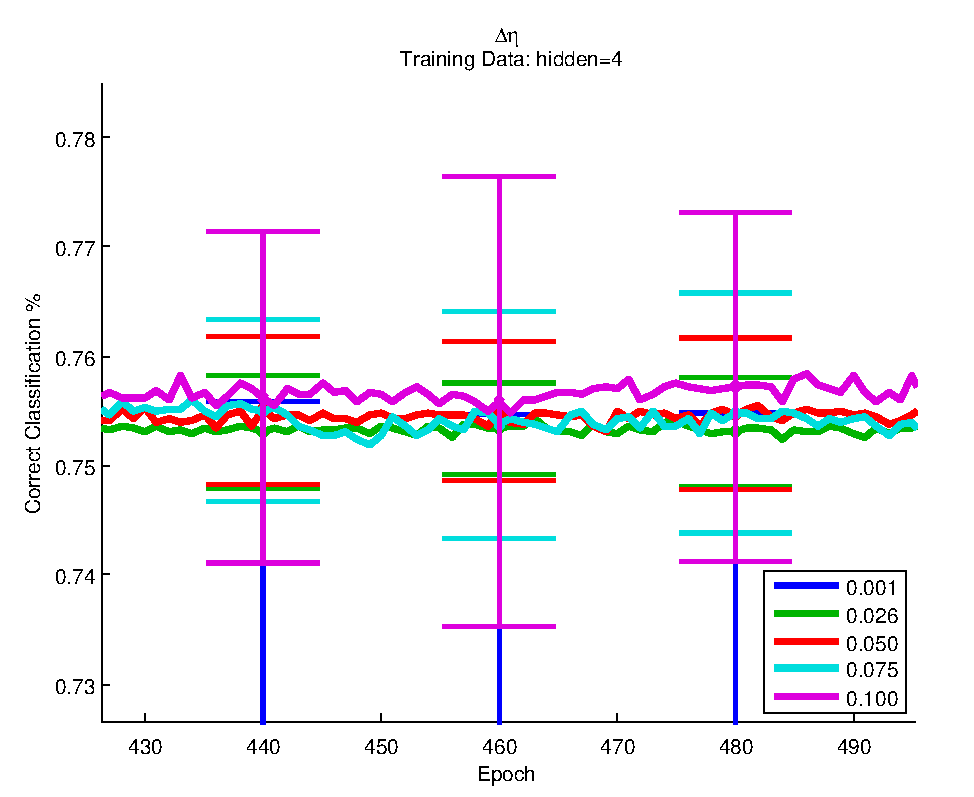
\includegraphics[scale=0.8]{../figures/eta_train_ex2.pdf}}
	\caption{	Focused graphs of \ref{fig:eTr} showing the variance between different
				learning rates ($\eta$). Although $\eta=0.1$ tended to end with a
				slightly higher average CCP, it had much greater variance between trials.
			}
	\label{fig:e1ex}
\end{figure}

\begin{figure}[bt]
	\vspace{-2 cm}
	\centering
	\subfigure[Detail of the beginning of figure \ref{fig:eT3}.]{\label{fig:eT3ex}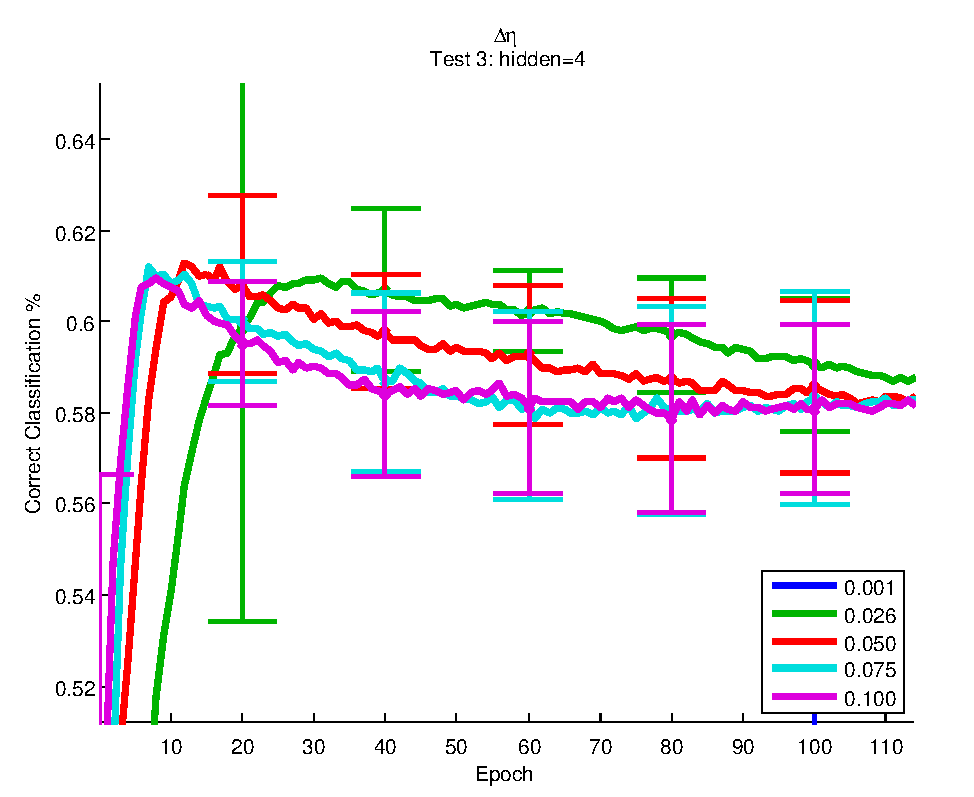
\includegraphics[scale=0.8]{../figures/eta_test3_ex.pdf}}
	\subfigure[Detail of the beginning of figure \ref{fig:eT3}.]{\label{fig:eT3ex2}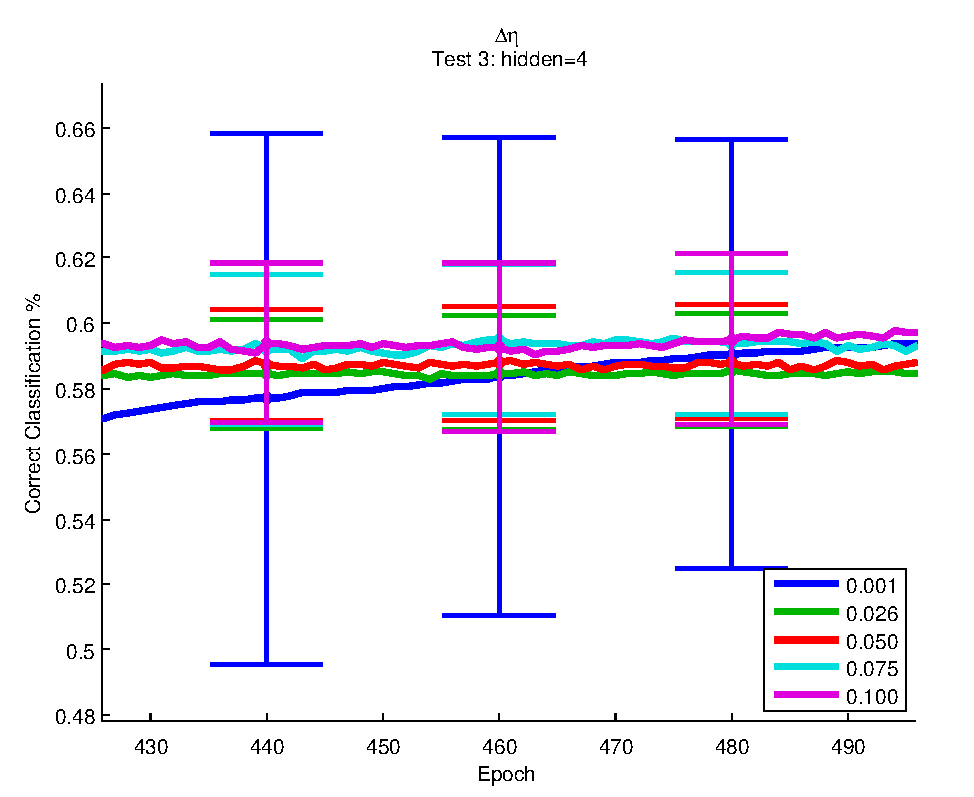
\includegraphics[scale=0.8]{../figures/eta_test3_ex2.pdf}}
	\caption{	Focused graphs of \ref{fig:eT3} showing the variance between different
				learning rates ($\eta$). Although $\eta=0.1$ tended to end with a
				slightly higher average CCP, it had much greater variance between trials.
			}
	\label{fig:e1ex2}
\end{figure}




\end{document}
